\subsection{Operational Risk and Resilience 相关概念}

\subsubsection{操作风险定义} 
\begin{itemize}
\item 运营风险被定义为因内部流程、人员和系统不足或失效或外部事件造成损失的风险。
    \begin{itemize}
    \item 该定义包括法律风险，但不包括战略和声誉风险。
    \item 然而，RPSMOR 于 2021 年发布： 在适当情况下，银行的操作风险管理应考虑战略和声誉风险。
    \end{itemize}
\end{itemize}




\subsubsection{操作风险分类}
\begin{itemize}
\item 内部欺诈（Internal fraud, IF）
    \begin{itemize}
    \item 内部欺诈是指公司员工实施或企图实施的欺诈行为。包括两个分项：
        \begin{itemize}
        \item 未经授权的活动
        \item 盗窃和欺诈（包括敲诈勒索、挪用公款、侵占资产、贿赂等）
        \end{itemize}
    \end{itemize}
\item 外部欺诈（External fraud, EF）
    \begin{itemize}
    \item 外部欺诈是指第三方或外部人员对企业实施或企图实施的欺诈行为，常见于零售企业。包括两个子项：
        \begin{itemize}
        \item 盗窃和欺诈（如支票拼凑和伪造）
        \item 系统安全（如黑客攻击）
        \end{itemize}
    \end{itemize}
\item 就业政策和工作场所安全性（Employment practices workplace safety , EPWS）
    \begin{itemize}
    \item 与欧洲或亚洲相比，美洲的就业惯例和工作场所安全（EPWS）类型更为突出，因为那里的劳动法比较陈旧，更多的是针对雇主的诉讼文化。包括三个分项目：
        \begin{itemize}
        \item 员工关系
        \item 安全环境
        \item 多样性和歧视
        \end{itemize}
    \end{itemize}
\item 客户、产品和业务操作
    \begin{itemize}
    \item 与客户和交易对手发生纠纷、因不当商业行为或错误咨询活动而被监管机构罚款所造成的损失。包括：
        \begin{itemize}
        \item 错误信息
        \item 投诉（complaints）
        \item 产品规格等错误招致的折扣贬损
        \end{itemize}
    \end{itemize}
\item 实物资产损害（Damage to physical assets, DPA）
    \begin{itemize}
    \item 涉及所有与自然灾害有关的损失事件以及来自恐怖主义和人为破坏等来源的人 为损失（故意破坏公共财物）。
    \item 这种风险最常用的评估方法是利用保险进行情景分析。
        \begin{itemize}
        \item 很少有公司主动收集这类风险的损失，因为这些损失通常要么太小，要么大得惊人
        \end{itemize}
    \end{itemize}
\item 业务中断和系统出错（Business disruption and system failures, BDSF）
    \begin{itemize}
    \item 业务中断或系统故障造成的损失最难发现。
        \begin{itemize}
        \item 例如，IT 故障、停电
        \end{itemize}
    \end{itemize}
\item 执行、交割和流程管理
    \begin{itemize}
    \item 交易处理失败造成的损失，以及与交易对手和供应商之间的问题
        \begin{itemize}
        \item 例如处理错误、文件缺失、供应商纠纷等。
        \end{itemize}
    \end{itemize}
\end{itemize}



\subsubsection{操作风险频率}


\begin{table}[h]
    \centering
    \caption{Event Categories with Frequency and Severity}
    \begin{tabular}{@{}>{\raggedright}ccc@{}}
        \toprule
        \textbf{Event category} & \textbf{Frequency} & \textbf{Severity} \\ \midrule
        Internal fraud - IF & 2\% & 2\% \\
        External fraud - EF & 30\% & 9\% \\
        Employment practices and workplace safety - EPWS & 15\% & 5\% \\
        Clients, products, and business practices - CPBP & 22\% & 52\% \\
        Damage to physical assets - DPA & 1\% & 1\% \\
        Business disruption and system failures - BDSF & 2\% & 5\% \\
        Execution, delivery, and process management - EDPM & 28\% & 27\% \\ \bottomrule
    \end{tabular}
\end{table}

\begin{itemize}
\item  CPBP 类别占不到四分之一事件频率造成的运营损失的一半以上。
\item EF、EPWS、CPBP 和 EDPM 占运营风险事件频率的 75%。
\item CPBP 和 EDPM 足以解释 79\% 的严重程度。
\item 值得注意的是，报告中的数字只反映了与每起操作风险事件相关的直接经济损失。
\item 大型操作风险事件的间接后果，如声誉受损、市值下降、管理层更替和补救成本，有时远远超过直接财务成本。
\end{itemize}

\subsubsection{操作风险的特点 }
\begin{itemize}
\item 异质性（Heterogenous）
    \begin{itemize}
    \item 操作风险是一系列不拘一格的风险，其成因和后果各不相同。即使在同一风险类别中，操作风险事件也可能大相径庭。
    \end{itemize}
\item 偶发性和扩散性
    \begin{itemize}
    \item EDPM 等操作风险类型由公司流程和系统的质量驱动或缓解。其他类型如 DPA 通常由外部事件引起。
    \end{itemize}
\item 重尾（heavy tailed）
    \begin{itemize}
    \item 业务风险以大量小额损失或少量巨额损失的形式出现。
    \end{itemize}   
\item 相互关联
    \begin{itemize}
    \item 不同类型的操作风险相互关联，因为它们可能有共同的内部原因，如内部控制薄弱、人为错误或风险文化不佳等。
    \end{itemize} 
\item 动态
    \begin{itemize}
    \item 许多业务风险的性质和强度取决于组织或行业的活动，并随着这些活动而变化。操作风险的演变与行业本身的发展相一致。
    \end{itemize}
\end{itemize}

\subsubsection{操作风险管理（ORM）框架}
\begin{itemize}
\item 代表所部署的行动、技术或工具。
\item 无论采用哪种表述方式，风险管理框架都将范围缩小到四项主要活动：
    \begin{itemize}
    \item 风险识别（risk identification）
    \item 风险评估（risk assessment）
    \item 风险缓解（risk mitigation）
    \item 风险报告（risk monitoring）
    \end{itemize}
\item 这四项活动通常以一个连续的循环来体现，以适应风险管理的迭代性质。
\item 风险管治涉及执行和报告风险管理的职责分配。
\item 风险文化和行为与获得每个人对风险管理和良好行为的认同有关。
\item 风险偏好和容忍度是对受监管金融服务公司的一项要求，以确定其在追求目标的过程中愿意面对的风险限度。
\end{itemize}


\subsubsection{运营复原力（Operational resilience）}
\begin{itemize}
\item 2010 年代后期，当金融部门和监管机构认为不仅需要关注金融稳定性，还需要关注运营稳定性，以及预防和从运营中断中恢复的能力时，对复原力的关注与日俱增。
\item 这种关注源于金融业对 IT 系统、基础设施和第三方供应商的严重依赖。
\item 英国发布首份运营弹性监管指南。英国金融行为监管局 (FCA)、审慎监管局 (PRA) 和英格兰银行 (BoE) 将运营复原力定义为：
    \begin{itemize}
    \item 企业和整个金融部门预防、适应、应对、恢复业务中断并从中学习的能力。
    \end{itemize}
\item 运营复原力的要素：
    \begin{itemize}
    \item 业务服务的连续性： 降低关键业务供应中断的风险。
    \item  重要（关键）业务服务： 一旦中断会对消费者或市场完整性造成不可容忍的损害的服务，并确保这些服务的连续性在可容忍的范围内。
    \item 影响容忍度： 发生事故时可容忍的中断程度，类似于业务连续性规划中的恢复时间目标。
        \begin{itemize}
        \item 影响容忍度必须包括基于时间的指标。
        \item 容限水平旨在帮助高级管理层和董事会制定自己的运营恢复能力标准，确定优先次序，并作出投资决定。
        \item 影响容许度的设定应假定会发生中断。
        \item 在设定单项重要业务服务的影响容限时，企业应考虑到其他相关重要业务服务故障的影响。
        \end{itemize}
    \item 中断管理： 应对中断、维护主要利益相关方的信任以及在危机时刻保持沟通的清晰度，是促 进系统稳定的重要因素。
    \item 吸取教训： 危机过后，可以从内部事故或其他公司的公共事件中吸取教训。
    \item 2020 年，美联储发布了《加强业务复原力的稳健做法》，并将业务复原力视为 ORM 不同组成部分的整体结果。
    \item ORM 是运营复原力的核心组成部分。
    \item ORM 有两个专业领域：第三方风险管理，这对供应链的复原力至关重要；情景分析，这是对尾随事件的必要准备。
    \item 业务连续性管理（BCM）和 IT 系统复原力是运营复原力的两个关键支持支柱。
    \end{itemize}
\end{itemize}




\subsection{Risk Governance}


\subsubsection{巴塞尔银行委员会健全 ORM 的原则}

\begin{itemize}
\item Pl: Culture led by the board of directors and implemented by senior management.
\item P2: Maintenance of a sound and proportionate ORM framework (ORMF).
\item P3: Board review and approval of ORMF.
\item P4: Risk Appetite and tolerance statement for operational risk
to be approved and periodically reviewed by the board.
\item P5: Senior management role in ORM policies and systems development and implementation.

\item P6: Comprehensive identification and assessment of operational risk in material activities.
\item P7: Change management process adequately resourced and
articulated.
\item P8: Regular monitoring of operational risk profile and exposures.
\item P9: Strong control environment: internal controls, mitigation, training, and risk-transfer strategies.
\item PlO: Robust information and communication technology (ICT) management program, in line with ORMF.
\item Pll: Business continuity plans in place and linked with ORMF.
\item P12: Public disclosures on approach to ORM and risk exposures.
\end{itemize}

\subsubsection{Supervisory expectation on governance of ORM}

\begin{itemize}
\item The fundamental expectation from regulators is that ORM should not be a mere compliance exercise of policies on paper, rubber-stamped by the governing body.
\item To protect against this risk of non-compliance, it is good practice to maintain a library of regulatory documents that govern how the operational risk framework should operate and ensure that all relevant staff are aware of their contents.
    \begin{itemize}
    \item Operational risk staff should be asked to confirm annually that they are fully aware of listed documents and contents.
    \end{itemize}
\end{itemize}

\begin{comment}
\begin{itemize}
    \item 监管机构的基本期望是，操作风险管理（ORM）不应仅仅是纸面政策的合规性工作，不能仅仅由管理机构盖章。
    \item 为了防止不合规的风险，维护一套监管文件库是良好的做法，这些文件规定了操作风险框架的运作方式，并确保所有相关员工都了解其内容。
        \begin{itemize}
        \item 操作风险工作人员应每年确认他们完全了解列出的文件及其内容。
        \end{itemize}
    \end{itemize}
\end{comment}


\subsubsection{Committee structure in risk governance}
\begin{itemize}
\item The lowest level oversees activity by business or function.
\item The group operational risk committee oversees, manages, monitors, and reports the consolidated picture to executive/management committee and board risk committee.
\item he board risk committee oversees all operational risk.
\item Operational risk is often split into several risk categories, with each category having its own committee in many large organizations, subordinated to:
    \begin{itemize}
    \item  either the board risk committee (or enterprise risk committee),
    \item or to the operational risk committee, reporting in turn to the enterprise risk committee.
    \end{itemize}
\end{itemize}


\subsubsection{Role of BOD in risk governance}

\begin{itemize}
\item The board of directors is ultimately responsible for:
    \begin{itemize}
    \item general administration of the firm.
    \item setting the risk appetite of the firm and for making sure that it operates within the limits of its risk appetite.
    \item establishing a risk management culture.
    \item validating the operational risk management framework and ensuring a periodic revision of the ORMF.
    \end{itemize}
\end{itemize}


\subsubsection{Three lines of defense model}
\begin{itemize}
\item Line 1: This is the risk owners understood as the front line of the business, so-called business unit management.
\item  Line 2: This is an independent corporate operational risk management function (CORF) which provides guidance, oversight and challenge of the first line.
\item  Line 3: This is the internal audit function serving as an independent assurance challenging line 1 and 2. Internal audit should report in solid line to non-executive directors.
\item Difference between line 1 and line 2: The first line owns the final sign-off on risks assessment and controls, this is not the role of the second line. The first line owns the risks and the second line owns the methodology.
\item  Line 1.5: Risk specialists (risk champions or risk correspondents or stewards) in each business department to interact with the risk function which are particularly common in larger organizations.
\end{itemize}


\subsubsection{Risk Appetite}
\begin{itemize}
\item  Definition: The board is responsible for determining and defining the nature and extent of the significant risks it is willing to take in achieving its strategic objectives.
\item It is the role of the board of directors to ultimately own the risk limits and to validate them periodically.
\item  In practice, the board often delegates this responsibility to the board risk committee, which in turn requests the support of the risk function to ensure the implementation of these limits in controls and exposure in the business, and to regularly report on them.
\item Risk appetite governance
    \begin{itemize}
    \item Allocate a risk owner to each risk type labeled in the risk appetite structure.
    \item  Designate control owners and metrics owners for the various operational risks when the risk appetite subcategories and controls cascade down into limits, controls, and monitoring metrics.
    \end{itemize}
\item Risk owners are responsible for managing, maintaining, and monitoring the risks with the stated limits of appetite and tolerance. Risk owners are the first line of defense.
\item  Controls owners are responsible for the design, implementation, and effectiveness of the controls.
\item  Metrics owners are responsible for the collection, reporting and monitoring of the metrics capturing the performance of the organization with regards to risk appetite.
\item Regulatory expectations for risk appetite
    \begin{itemize}
    \item  Easy to communicate and understand.
    \item  In alignment with the bank's strategy, business plans and operations of the firms.
    \item  Risk limits should be monitored through indicators related to risk exposure, control environment, and loss events.
    \item  Risk appetite should be forward-looking and subject to stress testing and have a view of what events might push the bank outside the limits of risk appetite and tolerance.
    \end{itemize}

\end{itemize}



\subsubsection{Definition of culture}


\begin{itemize}
\item Culture is the summation of values and ethics, desired conduct standards, and implied behaviors. While cultural norms and beliefs can't easily be measured, the conduct and behaviors that the culture norms can be observed, monitored, managed and incentivized. Conduct and behaviors are the only visible elements of culture.
\end{itemize}



\subsubsection{Risk culture}

\begin{itemize}
\item In the eyes of regulators, risk culture is closely associated with good conduct and ethics, and falls under the responsibilities of the board.
    \begin{itemize}
    \item Principle 1 by BCBS: The board of directors (BOD) should take the lead in establishing a strong risk management culture.
    \end{itemize}
\item The board of directors must lead the risk culture to be implemented by senior management. This is referred to as "tone at the top".
\item  Risk culture is supported by management reinforcement of:
    \begin{itemize}
    \item Codes of conduct and ethics.
    \item Compensation structure.
    \item Training to raise awareness of operational risks.
    \end{itemize}
\end{itemize}

\subsubsection{Risk culture-Codes of conduct and ethics}

\begin{itemize}
\item Reinforcement of adherence to the code of conduct and discipline are effective ways to influence behaviors.
    \begin{itemize}
    \item  But unnecessary blame should be avoided. A "no-blame culture" along with "tone from the top" is the most common recommendation for the establishment of a good risk culture.
    \end{itemize}
\end{itemize}

\subsubsection{Risk culture-Compensation structure}
\begin{itemize}
\item Toxic risk cultures are often triggered by overambitious shortterm growth and profit targets, undue pressure on staff and management, and resistance to bad news.
    \begin{itemize}
    \item Aggress1ve compensation structure like that the bank increases the proportion of incentive compensation for its traders and investment bankers should not be recommended.
    \end{itemize}
\end{itemize}



\subsubsection{Risk culture-Training}
\begin{itemize}
\item Common risk training programs include:
    \begin{itemize}
    \item induction training for new hires
    \item  online modules available to all staff
    \item  specialized training for the risk function
    \end{itemize}
\end{itemize}





\subsubsection{Signs of good risk culture}
\begin{itemize}
\item By experience, there are a handful of reliable signs of a healthy risk culture in organizations:
    \begin{itemize}
    \item  applicability of the rules to everyone
    \item  swift escalation of issues
    \item  sharing of the lessons learned
    \end{itemize}
\end{itemize}





\subsection{Risk Identification}

\begin{comment}
\begin{itemize}
\item 通过自上而下和自下而上的协调，可以全面了解操作风险状况。
\item Top-down: Start from the senior leadership, then down to business units, and finally to individual business processes.
    \begin{itemize}
    \item Target: Aim at identifying key organizational risks, the major business threats that could jeopardize strategic objectives.
    \item Outcome: Risk prioritization and risk ranking is an important outcome of top-down risk identification.
    \item  Tools:
        \begin{itemize}
        \item Business-specific risk identification
        
        Business-specific risk identification: exposures and vulnerabilities
            \begin{itemize}
            \item Exposure drives impacts in risk, should a failure materialize in one of these activities.
            \item  Vulnerabilities are the weakest links in business activities. These can be inadequate or outdated products, systems overdue for maintenance and testing, non-core businesses left unmonitored.
            \item If vulnerabilities are aligned with large exposures, this can result in very significant losses or a failure of the business.
            \item  The benefits of listing exposures and vulnerabilities as a risk identification brainstorming method has the main advantage of being business specific.
            \end{itemize}
        \item The risk wheel
            \begin{itemize}
            \item The risk wheel is a classic brainstorming tool to encourage creativity and ideas during risk identification workshops.
            \item  Domino effect: Salary cut down ➔personal effectiveness ➔ delays or descoping of project IT upgrade ➔ IT risk materializes ➔ systems disruption ➔ impact business continuity➔reputational damage.
            \end{itemize}
        \item Emerging risk identification: horizon scanning
            \begin{itemize}
            \item Known emerging risks: such as cyber, compliance, and climate change. In this, "emerging" means "increasing."
            \item  Nascent emerging risks: just starting to appear on the risk radar of a community or of an organization and truly deserve the term of emerging risk.
            \item  Benchmarking pieces of information can be used for inspiration or as a checklist.
            \item A way of scanning horizon risks is PESTLE analysis:
            
• Political

• Economic

• Social

• Technological

• Legal

• Environmental
            \end{itemize}
        \end{itemize}
    \end{itemize}
\item Bottom-up: It complements top-down approach. Businesses and divisions evaluate their own operational risk.
\end{itemize}
\end{comment}




\subsubsection{Scope of risk identification}
\begin{itemize}
\item Top-down: Start from the senior leadership, then down to business units, and finally to individual business processes.
\item Bottom-up: It complements top-down approach. Businesses and divisions evaluate their own operational risk.
\item 通过自上而下和自下而上的协调，可以全面了解操作风险状况。
\end{itemize}




\subsubsection{Top-down}

\begin{itemize}
\item Target: Aim at identifying key organizational risks, the major business threats that could jeopardize strategic objectives.
\item Outcome: Risk prioritization and risk ranking is an important outcome of top-down risk identification.
\item  Tools:
    \begin{itemize}
    \item Business-specific risk identification
    \item The risk wheel
    \item Emerging risk identification: horizon scanning   
    \end{itemize}
\item  Tools: Business-specific risk identification: exposures and vulnerabilities
    \begin{itemize}
    \item Exposure drives impacts in risk, should a failure materialize in one of these activities.
    \item  Vulnerabilities are the weakest links in business activities. These can be inadequate or outdated products, systems overdue for maintenance and testing, non-core businesses left unmonitored.
    \item If vulnerabilities are aligned with large exposures, this can result in very significant losses or a failure of the business.
    \item  The benefits of listing exposures and vulnerabilities as a risk identification brainstorming method has the main advantage of being business specific.
    \end{itemize}
\item Tools: The risk wheel
    \begin{itemize}
    \item The risk wheel is a classic brainstorming tool to encourage creativity and ideas during risk identification workshops.
    \item  Domino effect: Salary cut down ➔personal effectiveness ➔ delays or descoping of project IT upgrade ➔ IT risk materializes ➔ systems disruption ➔ impact business continuity➔reputational damage.
    \end{itemize}

\item Tools: Emerging risk identification: horizon scanning
    \begin{itemize}
    \item Known emerging risks: such as cyber, compliance, and climate change. In this, "emerging" means "increasing."
    \item  Nascent emerging risks: just starting to appear on the risk radar of a community or of an organization and truly deserve the term of emerging risk.
    \item  Benchmarking pieces of information can be used for inspiration or as a checklist.
    \item A way of scanning horizon risks is PESTLE analysis:
        \begin{itemize}
        \item  Political
        \item  Economic
        \item  Social
        \item  Technological
        \item  Legal
        \item  Environmental
        \end{itemize}
    \end{itemize}
\end{itemize}



\subsubsection{Bottom-up}
\begin{itemize}
\item Bottom-up risk identification tools
    \begin{itemize}
    \item Event and loss data analysis
    \item Risk and Control Self-Assessment (RCSA)
    \item Process mapping
    \end{itemize}
\item Event and loss data analysis
    \begin{itemize}
    \item Internal losses: Repeated internal losses might be a sign of failure in the internal controls system.
    \item  External losses: Such as consortium data. A best practice is to monitor all large incidents communicated by peers and ask objectively: "Could this incident happen to us?"
    \item  Near misses: Incidents that could have resulted in an operational loss but did not because of good luck or outside intervention. Near misses are "lessons for free".
    \end{itemize}
\item Risk and control self-assessment (RCSA):
    \begin{itemize}
    \item An organization, a business line, or a department evaluates the likelihood and the impact of its operational risks. This gives information on the level of residual risks.
    \item  RCSA is often workshop-style discussion facilitated by the second line to collect information from the first line.
    \item  In the largest institutions, the process can take the form of questionnaires.
    \item Selecting the relevant participants: Two types of employees are suitable to interview. One group is the most experienced employees. The other group comprises recent hires.
    \item  Frequency of RCSA: typically performed annually, updated after each trigger event in mature firms. If performed too frequently, the process can turn into a box-ticking exercise.
    \item The choice of the granularity of scope of RCSA workshops
        \begin{itemize}
        \item If too granular, the output will be a collection of small daily risks and inefficiencies that are not always of much value. People may miss the big picture when it comes to risks.
        \end{itemize}
    \end{itemize}
\item Process mapping: Lay out the tasks of a process, step by step, and asking what can go wrong in each step. This exercise highlights possible under-control or over-control of risks.
\item For process mapping, appropriate analysis is important:
    \begin{itemize}
    \item If too granular, the process mapping will be excessively time-consuming and likely to raise only minor issues.
    \item  If too high-level, it won't be informative enough to be used.
    \end{itemize}
\end{itemize}




\subsubsection{Scenario analysis- Brainstorming techniques}

\begin{itemize}
\item The regulatory guidance document describes scenario analysis as an exercise of extreme events identification, using workshops and brainstorming techniques.
    \begin{itemize}
    \item Brainstorming techniques are a method to identify, analyze and measure a range of scenarios, including low probability and high severity events.
    \end{itemize}
\item The preparation phase: Firms are required to minimize subjective biases when conducting scenario analysis.
    \begin{itemize}
    \item The participants in scenario analysis workshops should be senior managers within the different business functions with experience and understanding of the risks.
    \item  The involvement of additional external experts is advisable to help mitigate some biases such as myopia, excessive focus on scenarios driven by external causes.
    \end{itemize}
\item The generation phase aimed at producing a long list of scenarios to be considered.
\item  The intermediary phase: Scenario selection in which some scenarios are consolidated, and others eliminated or added.
    \begin{itemize}
    \item An example of consolidated scenarios are those relating to the same internal impact but different external causes.
    \end{itemize}
\item It is useful to compare the bank's scenarios with an industry scenarios, to determine whether omitting relevant scenarios.
\item  Some scenarios can be eliminated if the risk owner can convincingly demonstrate that the maximum loss generated by a given scenario is moderate enough to be absorbed by operating margin and without significant disruption.

\end{itemize}





\subsubsection{Examples of risk taxonomy}
\begin{itemize}
\item Basel taxonomy
    \begin{itemize}
    \item Level 1 is the highest-level category; level 2 is a detailed version of level 1; level 3 provides examples. The BCBS only recognizes the first two levels as regulatory categories.
    \item  The number of risks to assess, manage, and report needs to be kept at a reasonable level. Too much detail is detrimental to the quality of information, difficult to review, and can drain resources.
    \end{itemize}
\item Operational risk taxonomy by ORX
    \begin{itemize}
    \item The taxonomy revises the Basel operational risk taxonomy.
    \item  The taxonomy does not radically depart from the Basel categories but offers some noticeable modifications:
        \begin{itemize}
        \item It presents 14 level 1 risk types compared to 7 from Basel, and some level 2 risks have been elevated to level 1 given their prominence in today's world.
        \end{itemize}
    \end{itemize}
\end{itemize}



\subsubsection{Structure of taxonomies}
\begin{itemize}

\item Best practice is to distinguish and separately categorize the different components of uncertainties: causes, risks, impacts, and controls which are organized in taxonomies.
\item A structure of taxonomies of causes, controls, risks, and impacts, circling the actionable part of risk management: acting on the causes and the controls.
    \begin{itemize}
    \item Causes and controls are the prime objects of risk
    management actionability.
    \end{itemize}
\item It is neither reasonable nor economically efficient to attempt to eliminate every risk. However, trying to eliminate the downside of a risk while preserving its upside makes sense.
\item  To limit the downside of operational risk, organizations and individuals can, first, act on their causes and, next, apply controls on the remaining causes, to limit the two dimensions of a risk-the likelihood and the impact.
\item Cause taxonomy
    \begin{itemize}
    \item The natural level 1 causes for operational risk events by BCBS are PPSE, which is most common method adopted by the market.
    \item  But not every bank refines the categories to finer level 2 which provides useful insights into the causes of incidents.
    \end{itemize}
\item Impact Taxonomy
\begin{table}[h]
    \centering
    \caption{ORX Reference Impact Taxonomy}
    \begin{tabular}{@{}>{\raggedright}p{4cm}p{12cm}@{}}
        \toprule
        \textbf{Level 1} & \textbf{Level 2} \\ \midrule
        Direct financial impact & Such as timing loss, legal cost, damaged assets \\ \midrule
        Indirect financial impact & Such as opportunity costs, disruption \\ \midrule
        Non-financial impact & Stakeholder groups: customers, employees, third parties (vendors, suppliers, and service providers), shareholders, market/competition \\ \bottomrule
    \end{tabular}
\end{table}

\item Control taxonomy
    \begin{itemize}
    \item Preventative control
    \item  Detective control
    \item  Corrective control
    \item  Directive control
    \end{itemize}
\end{itemize}






\subsection{Risk Measurement and Assessment}


\subsubsection{Loss data collection}

\begin{itemize}
\item In 2000, ING created its first representation of the ORM framework. It comprised four concentric circles:

\begin{figure}[H]
    \centering
    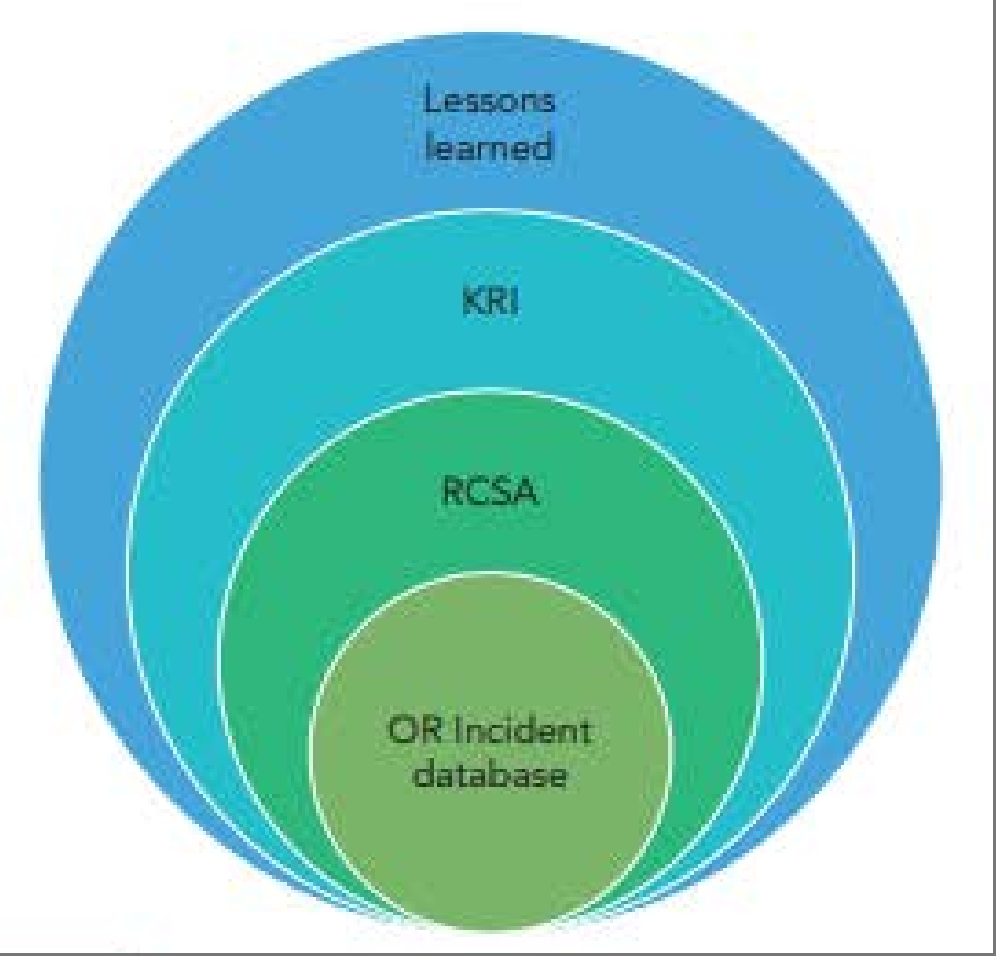
\includegraphics[width=0.3\textwidth]{images/frameworks0507.png}
    \caption{ORM framework}
    \label{fig:label1}
\end{figure}

\end{itemize}


\subsubsection{Incident database }

\begin{itemize}
\item Incident data collection (internal and external)
\item  Comprehensive data
\item  Dates of incidents and settlement lags
\item  Data quality requirements
\end{itemize}

\subsubsection{Comprehensiveness of data }
\begin{itemize}
\item Basel committee does not define "material activities and exposures," but sets a minimum threshold for loss reporting at €20,000 （about \$22,000）.
\item From a regulatory perspective, the choice of the reporting threshold should not affect the credibility of the process nor impair management information.
    \begin{itemize}
    \item It must be justified and should not suggest "cherry-picking " or manipulation of capital requirements.
    \end{itemize}
\item From a regulatory perspective, firms must only report incidents leading to financial losses.


\item  From a management perspective, it is good practice to record also the so-called "non-financial impacts," such as reputational damage, customer detriment, disruption of service, or management time and attention.
\item "Non-financial" impact is particularly misleading because the indirect consequences of many material operational risk events have financial implications: Regulatory scrutiny, customers'dissatisfaction, remediation plans, and management attention all have costly consequences.
    \begin{itemize}
    \item When these repercussions are not properly quantified, the cost of operational risk can be significantly underestimated.
    \end{itemize}
\item Grouped losses are distinct operational risk events connected through a common cause.
    \begin{itemize}
    \item Examples of grouped losses: the same wrong advice given to a group of clients, leading to a series of compensation
    claims.    
    \end{itemize}
\item Different events that materialize from a single failure must be grouped as a single loss to reflect the same underlying cause.
\end{itemize}




\subsubsection{Dates of incidents}
\begin{itemize}
\item Date of occurrence: when the event first happened
\item  Date of discovery: when it is first identified
\item  Date of reporting: when it enters the reporting database
\item  Date of accounting: when the financial impact enters the GL
\item  The difference between occurrence and discovery reflects the visibility of issues, whereas the difference between discovery and reporting shows how diligently operational incidents are reported to the risk function.
\item Include a maximum allowed time for reporting incident.
\item  Best practice dictates a risk-based approach that will not waste resources by rushing to report immaterial events.
    \begin{itemize}
    \item Material incidents must be reported within a few working days, while minor incidents can be included in periodic summary reporting.
    \end{itemize}

\item Reconciling the loss data recorded as operational losses with information from other sources. These sources often include the general ledger (GL) that captures all cash inflows and outflows of a firm, including unintentional losses and gains.
\item  GL is no substitute for a dedicated operational event database because it only captures the direct financial losses or accidental gains, but it does not link the indirect effects.
\item Underreporting is a challenge. Corporate incentives to report operational incidents range from soft encouragement to stringent oversight.
\item  Self-reporting of incidents is required, apply disciplinary action if unreported events are subsequently discovered. Most organizations include risk metrics in the balanced scorecard of their managers, as part of a risk-based performance system, a practice encouraged by regulators.



\end{itemize}


\subsubsection{Qualitative risk assessment}
\begin{itemize}
\item Risk and Control Self-Assessment (RCSA)
\item  Key performance indicators(KPls), Key risk indicators(KRls), Key control indicators(KCls)

\end{itemize}




\subsubsection{Risk and Control Self-Assessment (RCSA)}
\begin{itemize}
\item The RCSA refers to evaluating the likelihood and impact of operational risk faced by a business including both the firm's risk exposures before the impact of existing controls has been assessed (inherent risks), and those that remain after the evaluation of the controls in place (residual risks).
\item  Variations on the RCSA include the risk and control assessment (RCA) and the residual risk self-assessment (RRSA).
\item  RCSAs are qualitative and largely judgement-based.
\item  RCSAs are often conducted as workshop-style discussions.
\item  Some firms may form a dedicated risk assessment unit (RAU), responsible for the conduct of RCSAs. An RAU can be a part of a business line, division, or an organizational process.
\item  Mature organizations back-test the results of risk assessment against past incident experience.
\end{itemize}


\subsubsection{Severity assessment: impact scales}
\begin{itemize}
\item Four types of impacts: financial, regulatory, customer, and reputation.
\end{itemize}


\subsubsection{Likelihood assessment scales}
\begin{itemize}
\item Likelihood scales are either expressed in percentages of likelihood or frequency of occurrence （"once in x years"）.


\begin{table}[H]
    \centering
    \caption{Frequency of Occurrence and Probability Assessment}
    \begin{tabular}{|c|c|c|}
        \hline
        \textbf{Qualitative Rating} & \textbf{Frequency of Occurrence} & \textbf{Probability of Occurrence \% (one year horizon)} \\ \hline
        Likely & Once per year or more frequently & > 50\% \\ \hline
        Possible & > 1-5 years & 20-50\% \\ \hline
        Unlikely & 1 in 5-20 years & 5-20\% \\ \hline
        Remote & < 1 in 20 years & < 5\% \\ \hline
    \end{tabular}
\end{table}

\end{itemize}




\subsubsection{Combining likelihood and impact: heatmap }
\begin{itemize}
\item The various combinations of impact and likelihood are attributed colors that reflect the intensity of the risk. The colors used are red-amber-green or red-amber-yellow-green.

\begin{figure}[H]
    \centering
    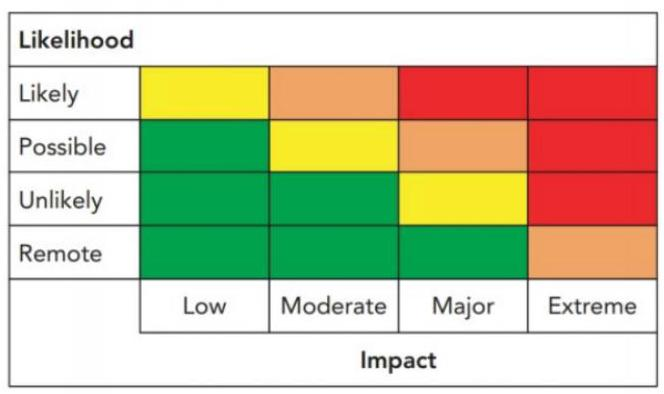
\includegraphics[width=0.3\textwidth]{images/heatmap.jpg}
    \caption{heatmap}
    \label{fig:label2}
\end{figure}

\end{itemize}


\subsubsection{Outcome of RCSA }
\begin{itemize}
\item The results of assessments must be documented and submitted to business line managers for approval and sign off.
\item  Action plans are owned by the first line (business-line managers) rather than the second line. Line managers are responsible for implementing mitigating action plans.
\item  Line managers and risk managers could expect to get from an RCSA exercise a view of residual exposure to key risks, when risks assessed as such are deemed above risk appetite, they will be the object of an action plan.
\end{itemize}


\subsubsection{Challenge of RCSA }
\begin{itemize}
\item The first challenge: Subjectivity of judgments, behavioral biases, and limited data input can quickly impede the quality and reliability of output.
\item  The second challenge: Difficulty in achieving comparable results across different assessment units, different departments, and businesses, often assessed by different people.
\end{itemize}


\subsubsection{Key Performance Indicators (KPI) }
\begin{itemize}
\item KPls measure performance or target achievement.
\item Examples of KPls include:
    \begin{itemize}
    \item Maximum downtime/uptime of IT systems
    \item  Error rates on retail transactions
    \item  Client satisfaction score/Level of client complaints
    
    \end{itemize}
\end{itemize}


\subsubsection{Key Risk Indicators (KRI) }
\begin{itemize}
\item KRIs are monitoring metrics that signal the increase/decrease in the level of risk, either in potential impact or in likelihood.
\item  Examples of KRIs used in measuring likelihood include:
    \begin{itemize}
    \item  Increase in number of transactions per staff (risk of errors)
    \item  Drop in customer satisfaction scores (risk of client attrition)
    \item  Increase in the level of sales required for sales staff to achieve a performance objective (risk of fraud)
    
    \end{itemize}
\item Examples of KRls measuring impact include:
    \begin{itemize}
    \item Increase in the level of proprietary company knowledge held by a key employee （higher impact of discontinuity/loss of knowledge in case of departure/ sickness）
    \item  Increase in sensitivity of data held on given server （higher impact in case of data leakage/loss）
    \item  Increase in value generated by top-10 clients （higher impact in case of client attrition）
    \end{itemize}

\end{itemize}

\subsubsection{Key Control Indicators (KCI) }
\begin{itemize}
\item Key control indicators (KCls) measure the effectiveness of controls, either in design or performance. Examples of KCls:
    \begin{itemize}
    \item Missed due diligence items
    \item  Lack of segregation of duties
    \item  Overlooked errors in four-eye checks (reviews by two competent individuals)
    \end{itemize}
\end{itemize}

\subsubsection{Interaction among KPls, KRls, and KCls }
\begin{itemize}
\item KPls, KRls, and KCls overlap in many instances, especially when they signal breaches of minimum standards.
\item  The failure of a control function is jointly a KPI, a KRI, and a KCI.
    \begin{itemize}
    \item  A poor performance will often become a source of risk.
    \item  A key control failure always constitutes a source of risk.
    \end{itemize}

\item  KRI thresholds and governance reflect the risk appetite and tolerance levels of an organization.
\end{itemize}

\subsubsection{Quantitative risk assessment}
\begin{itemize}
\item Causal analysis of scenarios
\item  Fault Tree Analysis (FTA)
\item  FAIR methodology
\item  Root-cause analysis and Bowtie tool
\item  Swiss cheese: control layering
\end{itemize}

\subsubsection{Causal analysis of scenarios}
\begin{itemize}
\item Causal analysis is used to quantify operational risk scenarios, which focuses on tails (rare events) that affects the firm significantly.
\item  Causal analysis is based on forward-looking (not past) determinants of impacts and likelihood of operational risks.
\item  Quantitative risk assessment is important but challenging task in risk management when it comes to scenarios.
\end{itemize}

\subsubsection{Fault Tree Analysis (FTA)}
\begin{itemize}
\item Fault trees decompose failure scenarios into external conditions and internal conditions.
\item FTA is built upon a series of conditions that can either happen simultaneously (known as "AND conditions") or alternatively (known as "OR conditions").

\begin{figure}[H]
    \centering
    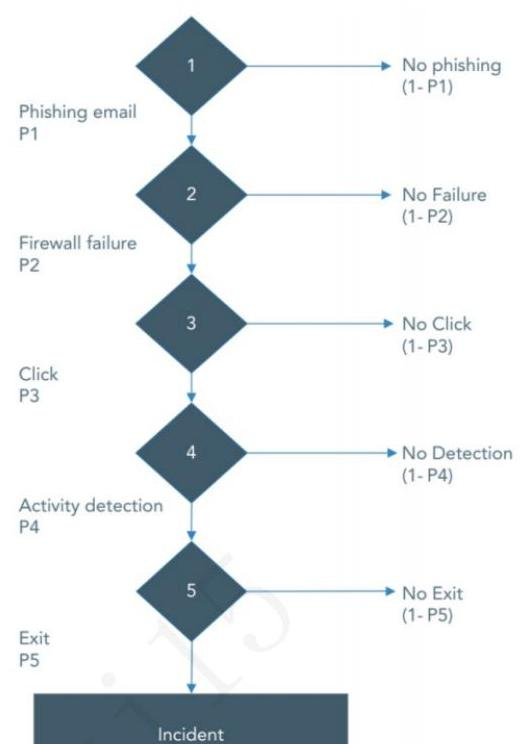
\includegraphics[width=0.3\textwidth]{images/FTA.jpg}
    \caption{FTA}
    \label{fig:label3}
\end{figure}

\item If conditions are independent, likelihood of this risk materializing is: Pl *P2*P3*P4*PS.
\item  If control failures and other impact factors are dependent: Bayesian (conditional) probabilities.

    \begin{itemize}
    \item Bayesian models refer to measurement methods where likelihood assessments are updated by new information.
    \end{itemize}

\end{itemize}


\subsubsection{FAIR methodology}
\begin{itemize}
\item FAIR (factor analysis of information risk) is a factor model for quantifying operational risk, which is based on decomposition of the risk into their factors.
\item  The steps are as follows:
    \begin{enumerate}
    \item   Identification of the risk factors and interrelationships
    \item   Measurement/metric of each factor
    \item   Computational combination of the factors
    \end{enumerate}
\item In this method, a scenario should have:
    \begin{itemize}
    \item an asset at risk (asset of the scenario)
    \item a threat community (who or what the threat is)
    \item a threat type (nature of the threat)
    \item an effect (losses resulting from materialization of the risk)
    \end{itemize}
\end{itemize}


\subsubsection{Root-cause analysis and Bowtie tool}
\begin{itemize}
\item It takes the form of the "5-why" analysis. Recommendations require the first line to perform root-cause analysis. The investitzations should be challeneed bv the second line.

\begin{figure}[H]
    \centering
    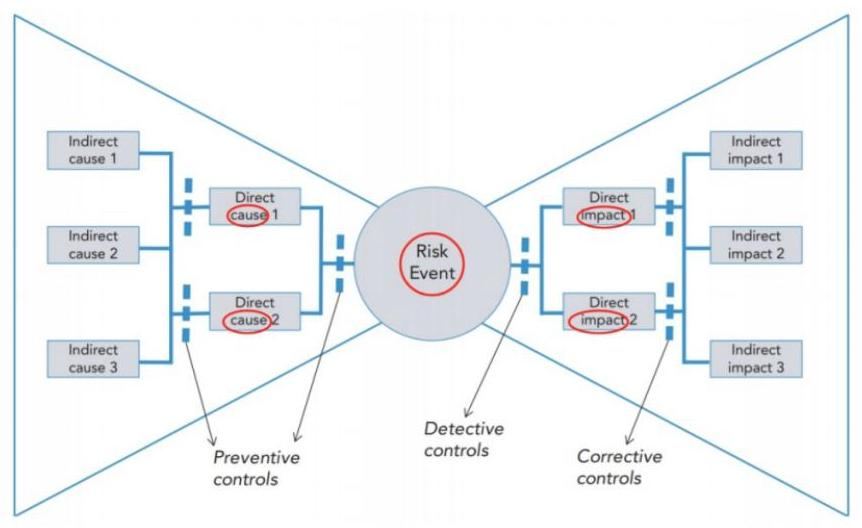
\includegraphics[width=0.3\textwidth]{images/RISKEVENT.jpg}
    \caption{RISKEVENT}
    \label{fig:label4}
\end{figure}


\item Bowtie analysis is useful for:
    \begin{itemize}
    \item assessment of the likelihood and impact of risks.
    \item better understanding of the causes of risks and the possible failure of controls that may lead to their materialization.
    \item investigating how quickly an incident is detected and how well the organization reacted in limiting the impacts.
    \end{itemize}
\end{itemize}


\subsubsection{Swiss cheese: control layering}
\begin{itemize}
\item It is also called the cumulative act model. Each defensive layer are like slices of Swiss cheese, having many holes, which are continually opening, shutting, and shifting their location. The presence of one hole does not cause a bad outcome but does when holes in many layers momentarily line up.


\begin{figure}[H]
    \centering
    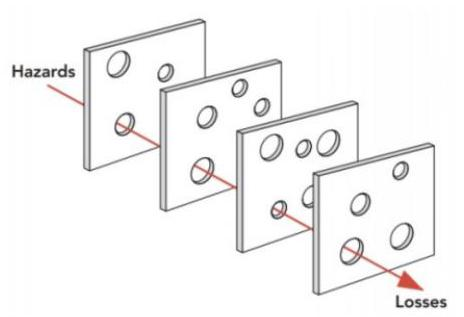
\includegraphics[width=0.3\textwidth]{images/Swisscheese.jpg}
    \caption{Swisscheese}
    \label{fig:label5}
\end{figure}

\item  In an effective control layering, where the holes are not aligned (failure rates of controls are independent), and controls compensate each other's weaknesses to produce a control system that works as a tight safety net, rather than like a row of dominos.
\item  Assessing independence of controls is at least as important as assessing reliability of each individual control.

\end{itemize}


\subsubsection{Operational risks modeling and capital}
\begin{itemize}
\item Loss Distribution Approach (LDA): Advanced Measurement Approach (AMA)
    \begin{itemize}
    \item Frequency (discrete) is modeled with Poisson distribution and negative binomial distributions.
    \item  Severity (continuous) is modeled with log-normal distribution, Weibull and Generalized Pareto Distributions (GPD) (More heavy-tailed).
    \item Regulators require clear rules to be set for the selection of data and avoid "cherry picking" and manipulation of results.
    \item  Internal loss data is the backbone of LDA because of more relevant to the organization.
    \item  External loss data from peers can be supplemented.
    \item  Mix internal and external data: Scale, Cut-off mix, Filter. 
    \end{itemize}
\item Limitations and constraints of LDA 
    \begin{itemize}
    \item The distributions of severity and frequency of operational losses are typically assumed to be independent.
    \item  Data are split into risk classes (or units of measure), where losses within each risk class should be iid (independent and identically distributed).
    \end{itemize}
\item LDA modeling Pillar 1 of regulatory capital are now being transferred to modeling Pillar 2 under ICAAP (Europe), as well as stress-testing calculations (USA) and operational resilience.
    \begin{itemize}
    \item The ICAAP is part of Pillar 2 of regulatory requirements which covers all financial and non-financial. So, ICAAP applies to all risks, not only operational risk.
    \item  The ICAAP can inform the economic capital and both have the same purpose.
    \end{itemize}
\end{itemize}


\subsubsection{Quantification of operational resilience }
\begin{itemize}
\item Differences between resilience frameworks and traditional business continuity management (BCM)
    \begin{itemize}
    \item BCM focuses on the continuity of each business process and recovery, in case of disruption within a given time frame (Recovery Time Objective, RTO).
    \item  Resilience focuses on the continuity and recovery of important business services.
    \end{itemize}
\item Key steps for operational resilience



\begin{figure}[H]
    \centering
    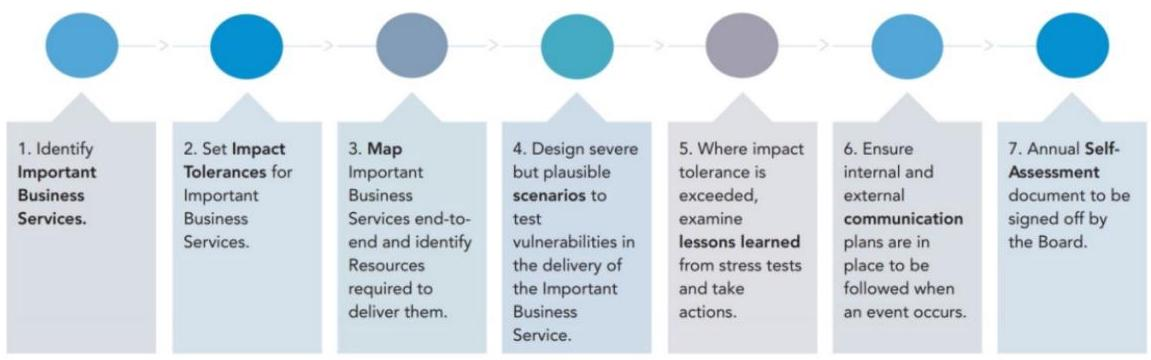
\includegraphics[width=0.8\textwidth]{images/keysteps.jpg}
    \caption{keysteps}
    \label{fig:label6}
\end{figure}


\item Impact tolerances can be built up through business impact analysis (BIA). BIA is the assessment of consequences of disruption of a process or a service in business terms, but also on the resources needed to develop recovery strategies.
\item  The BIA report should prioritize the order of events for restoration. Business processes with the greatest operational and financial impacts should be restored first.
\item  Single points of failure (SPOF) are relevant KRls for resilience.
    \begin{itemize}
    \item One example of KRls is the number of key employees without back-ups, without documented processes, with unique knowledge and skills.
    \item  SPOF need to be mitigated and removed through back-up and redundancies, and if not, they need to be considered when setting tolerance thresholds and stress tests.
    \end{itemize}
\end{itemize}





    
\subsection{Risk Mitigation}



\subsubsection{Two kinds of operational risk}
\begin{itemize}
\item Operational risks can be categorized in two types:
    \begin{itemize}
    \item External operational risks are those that arise due to the business environment of the organization or due to external events. External operational risks cannot be prevented, but they can be reduced.
    \item Internal operational risks are linked to people, processes, and systems. Internal operational risks tend to be far more preventable, largely through the use of internal controls.
    
    \end{itemize}
\end{itemize}


\subsubsection{Risk response}
\begin{itemize}
\item Tolerate: accepting the risk as it is.
\item Treat: encapsulating all the types of risk mitigation, mostly internal controls.
\item Transfer: moving the risk to another party (external insurance).
\item Terminate: removal of all risk exposure by discontinuing a product or ceasing operations in certain countries
\end{itemize}


\subsubsection{Internal control types}
\begin{itemize}
\item Preventive controls: intended to reduce the likelihood of an incident.
    \begin{itemize}
    \item Segregation of duties
        \begin{itemize}
        \item The front-office (trading desk) initiates trades, validated by the middle-office, confirmed and settled in the backoffice and treasury departments.
        \end{itemize}
    \item  Access controls (digital or physical)
    \item  Levels of authorization
    \item  Process automation
    \end{itemize}
\item Detective controls: designed to alert if an incident occurs, accelerate its resolution, and limit the impact of the incident to the firm or its stakeholders.
    \begin{itemize}
    \item Exception reports
    \item  File reconciliations
    \item  Smoke detectors
    \item  Intrusion detection systems
    \end{itemize}


\item Corrective controls: mitigating technique designed to lessen the impact to the institution when adverse events occur. They do not influence the likelihood of a risk happening, but lessen the pain if it does.
    \begin{itemize}
    \item  Data back-ups
    \item  IT systems patch management
    \item  Continuity planning
    \item  Systems redundancies
    
    \end{itemize}
\item Directive controls: include all the prescriptions and rules to execute a process.
    \begin{itemize}
    \item Procedures and guidance manuals
    \item  Internal training
    \item  Team supervision
    \item  Handover procedures
    \end{itemize}
\end{itemize}


\subsubsection{Control design}
\begin{itemize}
\item Types of weakly designed controls include the following:
    \begin{itemize}
    \item  Optimistic controls
    
    Such as sign-offs for large volumes of documents before  a deadline.
    \item  Collective controls
    
    Such as "four-eyes check" diluting accountability.
    \item  More of the same
    
    Such as responding to a failure of collective controls by
    adding more controllers.
    \end{itemize}
\end{itemize}


\subsubsection{Control testing}
\begin{itemize}
\item The main types of control testing are the following:
    \begin{itemize}
    \item Self-certification or inquiry: limited to secondary controls or controls related to low risk environments.
    \item  Examination: This requires supporting evidence and documentation. The effectiveness depends on the relevance and adequacy of the documentation. It provides moderate assurance and is better suited for automated controls and sampling of manual controls.
    \item Observation: involves real-time oversight of the execution of the control process to judge its design and effectiveness.
    \item  Reperformance: also called reproduction or parallel testing. The tester reproduces the control process on a sample of transactions and compares the results with those previously obtained by the process. It is the strongest form of testing.
    \end{itemize}
\end{itemize}


\subsubsection{Risk mitigation by process design}
\begin{itemize}
\item Prevention through design
    \begin{itemize}
    \item Examples include checklists, communication protocols, standardization, and optimized work environments or
    systems design.
    \end{itemize}
\item Typology and mitigation of human error
\item  Lean Six Sigma
\item  Quality improvement
\item Lean Six Sigma: DMAIC cycle

\begin{figure}[H]
    \centering
    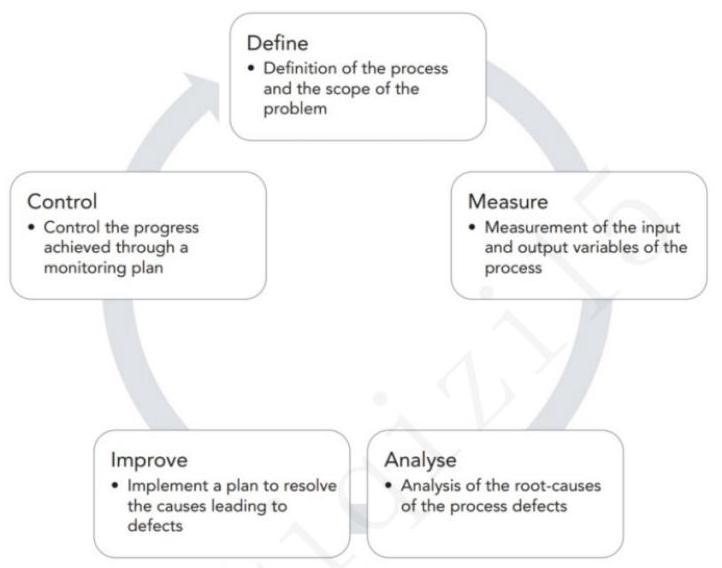
\includegraphics[width=0.5\textwidth]{images/DMAIC.jpg}
    \caption{DMAIC}
    \label{fig:label7}
\end{figure}


\item Quality improvement: represented by PDSA cycle.
    \begin{itemize}
    \item Plan: objective; questions and predictions; develop a plan to improve the model (who, what, where, when)
    \item  Do: carry out the plan; document problems and unexpected observations; begin data analysis
    \item  Study: complete the data analysis; compare data to predictions; summarize what was learned
    \item  Act: what changes are to be made? next cycle?
    \end{itemize}


\end{itemize}



\subsubsection{Typology and mitigation of human error}
\begin{itemize}
\item  Four kinds of human error
    \begin{itemize}
    \item Skilled-based: slip
        \begin{itemize}
        \item Involuntary
        \item  Caused by inattention, distraction, environment, tiredness.
        \item  Controls: Improved, supportive environment, re-engineered processes, adjusted pace, etc.
        \end{itemize}
    \item Rule-based: mistakes
        \begin{itemize}
        \item Wrong action based on flawed rules
        \item  Caused by wrong incentives, flawed products, misleading instructions, etc. One example is mis-selling to customers due to aggressive commercial incentives.
        \item  Controls: change the rule
        \end{itemize}
    \item Knowledge-based: mistakes
        \begin{itemize}
        \item Wrong choice of action facing a new situation
        \item  Caused by lack of training, knowledge of the environment, causes and/or consequences of actions
        \item  Controls: training, documented procedures, help file, escalation rules
        \end{itemize}

    \item A fourth type is a violation
        \begin{itemize}
        \item Voluntary misdeed
        \item  Controls for violations: Supervisory controls, either human or automated, through hierarchy, cameras, or automated recordings, improvements in risk and compliance culture that reward adherence to rules and processes
        
        \end{itemize}
    \end{itemize}
    
\end{itemize}



\subsubsection{New Product approval process}
\begin{itemize}
\item Every project, product, and initiative in a business will bring novelty, lack of familiarity, and uncertainties that may generate significant operational risks.
\item  A common risk-mitigation approach is the New Product Approval Process (NPAP), and its generalization to new initiatives, New Initiative Risk Assessment Process (NIRAP).
\item Best practice requires to present a business case to justify the allocation of resources. A proper business case would cover at
a minimum five topics:
    \begin{itemize}
    \item Objective: what we want the firm to achieve and the rationale for the project.
    \item  Alternative: Other options considered and reasons for selecting the current project.
    \end{itemize}

\item A proper business case would cover at a minimum five topics:
    \begin{itemize}
    \item Expected benefits: Expected benefits and synergies from the project, and possible drawbacks.
    \item  Commercial aspects: The costs, investment needs, and funding arrangements.
    \item  Risks: Main risks and their possible impact on the business case and on the rest of the business, with their mitigation.
    \end{itemize}
    
\item Stages of involvement of risk function during a project's life.

    \begin{itemize}
    \item Initial stage (before kick-off):
        \begin{itemize}
        \item Risk identification and assessment
        \item Mitigation and monitoring plans
        \end{itemize}
    \item Project life:
        \begin{itemize}
        \item monitoring and risk update, regular meetings with the risk team and the project team to update risk identification and assessment findings for important and critical projects.
        \end{itemize}
    \item Project closure:
        \begin{itemize}
        \item Debriefing, evaluations of project deliverables, analysis and documentation of the risks, lessons learned. 
        \end{itemize}
    \end{itemize}

\end{itemize}


\subsubsection{Mitigation measures to reduce impact}
\begin{itemize}
\item Key measures of impact reduction:
    \begin{itemize}
    \item Contingency planning (Plan B)
    \item Resilience measurement
    \item Crisis management and communication
    \end{itemize} 
\end{itemize}


\subsubsection{Contingency planning }
\begin{itemize}
\item Contingency planning is a component of business continuity, disaster recovery, and of corrective risk management, the planning phase of corrective and directive controls.
\item  Specific forms of contingency planning are business continuity management (BCM) and disaster recovery plans (DRP). These are most relevant when we consider operational resilience
\item To be effective, the plan needs to be regularly tested, to ensure the practicality and speed of its implementation in case of an emergency.
\item  There must be a key owner who has clear responsibility for the design of actions and their execution, including communication with outside parties
\item BCM as an ongoing process
    \begin{itemize}
    \item The first step is to ensure senior level commitment. Topdown direction, support, and ownership are essential in both the BCM process and the quick activation of the BCP when a crisis hits.
    \item The next step is to initiate the management process and identify a team to take ownership as a continuing project,
    rather than a one-off event.
    \end{itemize}
    
\end{itemize}


\subsubsection{Event and crisis management}
\begin{itemize}
\item To manage a crisis or a large operational event effectively
    \begin{itemize}
    \item Speed
    \item  Competence
    \item  Transparency
    \end{itemize}
\item In crisis model, firms should have at a minimum two types of incident response teams:
    \begin{itemize}
    \item A technical team (or recovery team), composed of specialists who assess the incident and focus on restoring normal processes as quickly as possible.
    \item  A communication team (external or internal), which deals with the media and the different stakeholder groups, including employees.
    \end{itemize}
\item Four typical phases of a major operational risk event:
    \begin{itemize}
    \item Crisis
    \item  Emergency response
    \item  Recovery (RPO and RTO)
    \item  Restoration (back-to-normal)
    
    \end{itemize}
\item Recovery Point Objective (RPO) indicates the amount of data updated or created that will be lost or need to be re-entered after an outage.
\item Recovery Time Objective (RTO) is the amount of downtime a business can tolerate. The RTO is the maximum tolerable duration of disruption for a process, a system, or a service.
\end{itemize}


\subsubsection{Risk transfer}
\begin{itemize}
\item Two methods to transfer risks:
    \begin{itemize}
    \item External Insurance: An organization agrees to pay a regular premium in exchange for being compensated should a certain risk materialize.
    \item  Outsourcing: The process of delegating some of the company's tasks to a third party under a contractual agreement, such as IT server management, cloud computing, data centers, or call centers.
    \end{itemize}
\end{itemize}


\subsubsection{Risk transfer-external insurance}
\begin{itemize}
\item For small losses: Many large institutions either self-insure small losses via a captive subsidiary or just absorb the volatility.
\item  For large losses: Financial institutions mainly use external insurance to cover extreme operational risk "tail" events, such as cyber risks, business discontinuity, or major class action lawsuits.

\end{itemize}


\subsubsection{Risk transfer-outsourcing }
\begin{itemize}
\item For traditional banks: internalize credit decisions and allocations but outsource some of their ICT activities.
\item  For FinTech banks: more likely to manage their own technology platforms, but outsource credit risk decisions to other specialists.
\item Outsourcing can increase or decrease the risk for an organization. depending on what process or activity is outsourced, to whom, and for which reasons.
\item  Outsourcing can result in increased operational risk labeled third-party risk. Increasingly, outsourcing is seen as a "risk sharing" activity.
\end{itemize}



\subsubsection{Management of reputational risk}
\begin{itemize}
\item Important elements such as reputational damage cannot really be outsourced (nor repaired) through insurance.
\item Therefore, prevention and mitigation strategies are essential to build a solid reputation and to react quickly and appropriately in times of crisis to limit reputational damage following operational risk incidents.
\item Some preventive controls and strategies are designed to build and maintain customer confidence.
\item Detective controls, such as monitoring customer complaints on social media and tracking trends in refund requests or system downtimes, are designed to identify operational failures but also reduce their reputational impact.
\item Many corrective risk controls and mitigation strategies are in place to protect the company's reputation and form actions taken when operational events hurt customers.
\end{itemize}



\subsection{Risk Reporting}





\subsubsection{Roles and responsibilities of committees}
\begin{itemize}
\item Risk Committee
    \begin{itemize}
    \item Risk committee is authorized by the board to monitor the effectiveness of risk management framework.
    \item  The risk committee will receive information on key risk indicators associated with the firm's risk appetite, the frequency and severity of risk events, and the investigation of the causes of large events etc.
    \item  Any significant issues in control system or in operational risk status will be escalated to the risk committee.
    \item Reporting requirements related to the firm's operations must be sufficient for the board risk committee to determine that the organization's control and monitoring systems can effectively comply with, and operate within limits of, the firm's risk appetite, which is set by the board.
    
    \end{itemize}
\item Executive committee (ExCo)
    \begin{itemize}
    \item Composed of elected board members and senior executives, acting as a steering committee for board.
    \item  Facilitate decision-making during times of crisis and prioritize issues for the board to address during normal time.
    \item  Oversee board policies, and ensure good governance practices.
    \item  Oversee effective execution of the ORM framework. 
    \end{itemize}
    
\item Audit committee
    \begin{itemize}
    \item Responsible for a third level of operational risk oversight managed by the firm's internal audit activities (the third line of defense).
    \item  Responsible for the assurance on the internal control system of the organization.
    \item Internal audit and audit committee have several crossovers with respect to ORM activities.
        \begin{itemize}
        \item Internal audit function regularly audits operational risk function and report findings to ExCo and audit committee.
        \item  Vulnerabilities in the control systems uncovered through internal audits are reported to audit committee.
        
        \end{itemize}
    \end{itemize}
\item Operational risk committee
    \begin{itemize}
    \item Central ORM function as a second line of defense centralizes most information regarding operational risk and its management.
    \item Central ORM function provide an aggregated view of various risks which are often managed in a siloed manner at the business-line level and their interaction.
    \item Central ORM function collects all relevant operational risk information from business lines to produce aggregated, synthesized reporting for operational risk committee and provide feedback to business lines, enabling them to:
        \begin{itemize}
        \item monitor their own operational risks.
        \item benchmark their performance relative to other business lines or departments, or to a firm-wide average.
        \end{itemize}
    
    \end{itemize}


\end{itemize}



\subsubsection{Considerations of operational reporting}
\begin{itemize}
\item Reports should be neither too large nor too small.
    \begin{itemize}
    \item If too large: significant risk of overlooking key pieces of information. Too much information can bury key insights.
    \item If too small: it can become meaningless.
    \end{itemize}
\item There is little uniformity in operational reporting across firms:
    \begin{itemize}
    \item Some focus on narrative of past risk events, others focus on forward-looking indicators. The more mature the ORM approach, the more forward-looking its reporting.
    \end{itemize}
\end{itemize}



\subsubsection{Seven elements of internal ORM report}
\begin{itemize}
\item Seven elements included in internal ORM report:
    \begin{enumerate}
    \item Top-10 risks and risk outlook in risk inventory
    \item Heatmap and risk register
    \item Risk appetite metrics
    \item KRIs and issue monitoring
    \item Incidents and near misses
    \item Action plans and follow-up
    \item Emerging risks and horizon scan finding
    \end{enumerate}
\item Risk appetite metrics
    \begin{itemize}
    \item Risk appetite metrics (or risk appetite KRls) are indicators reflecting the firm's compliance with risk limits for its operational risk appetite.
    \item At the business level, these metrics are collected and analyzed individually.
    \item When reported to upper levels of management and board, risk appetite metrics are presented as a single list.
    \end{itemize}
\item KRIs and issue monitoring
    \begin{itemize}
    \item KRIs can provide a granular, forward-looking analysis of risk exposure in different activities.
    \item Issues are grouped by business line or a major initiative (new business, merger etc.) to make reporting actionable.
    \end{itemize}
\item Incidents and near misses
    \begin{itemize}
    \item Increasingly, loss classifications are standardized and shared across financial institutions. One common standard is the ORX global banking loss-data service classification.
        \begin{itemize}
        \item Although increasingly standardized, reporting thresholds may vary widely from firm to firm.
        \end{itemize}
    \item The materiality of an operational risk event must be judged not only by actual impact but also by potential impact.
        \begin{itemize}
        \item Reporting thresholds for risk events and near misses should theoretically be based on potential impact of the event rather than its materialized impact.
        \item Given the difficulty to estimate potential impact, firms and regulators use observed impact to set reporting thresholds.
        
        \end{itemize}
    \end{itemize}
\item Action plans and follow-up
    \begin{itemize}
    \item Action plans (including preventive, detective and corrective action plans) are risk-mitigation programs designed to improve the control environment.
    \item Action plans are tracked, reported by business-line owner.
    \item There is a zero objective for firms where risk management is strong: zero overdue actions and zero overdue audit recommendations.
    \end{itemize}
\item Emerging risks and horizon scan finding
    \begin{itemize}
    \item In a volatile environment, practice of horizon scanning to identify new trends and emerging risks has been instituted.
        \begin{itemize}
        \item Emerging risks are reported regularly to risk committee.
        \item Much of horizon scanning focuses on regulatory risks and changes in the compliance and regulatory environment.
        \item Best practices suggest horizon scanning should reflect elements that could cause change in emerging risks.
        \end{itemize}
        
    \end{itemize}



\end{itemize}



\subsubsection{Characteristics and challenges of operational risk data}
\begin{itemize}
\item Operational loss data are:
    \begin{itemize}
    \item heavy tailed or skewed statistically away from the mean.
    \item asymmetry with small number of large loss but large number of small losses
    \end{itemize}
\item A proper allocation of risk management resources is to focus on the prevention and remediation of large incidents and not to be dispersed and distracted by daily volatility
\end{itemize}



\subsubsection{Ways to overcome these challenges}
\begin{itemize}
\item Escalation of large risk events to upper management.
\item Identify and analyze regularly large number of small losses.

    
\item Benchmarking operational losses
    \begin{itemize}
    \item Reporting operational losses as a percentage of gross income, of total cost, total budget, or in basis points of capital facilitates the comparability.
    
    \end{itemize}
    
\item No averages because of its asymmetric distributions
    \begin{itemize}
    \item Averages hide the heterogeneity. The bias in operational loss averages is often caused by outliers.
    \item Better alternatives to averages are the median and the first and third quartiles of the distribution.
    
    \end{itemize}
    
\item Combined assurance: The three lines of defense should work together to provide combined assurance to the board (RAG).

\end{itemize}




\subsubsection{Aggregating qualitative risk data}
\begin{itemize}
\item The challenge is that risk scores, color ratings, and other indicators are discrete, qualitative, unfit for arithmetic treatment. Solution includes:
    \begin{itemize}
    \item Conversion and addition
    \item Categorization
    \item Worst-case reporting
    
    \end{itemize}
\item Conversion and addition: Convert qualitative metrics into monetary unit that is linear, additive arithmetically.
\item Categor1zat1on: Grouping them by color or score avoids the misleading collapse of heterogeneous information into improper aggregate.
\item Worst-case reporting: Conservatism and prudent form, appropriate when risk tolerance is minimal, disadvantage is potentially over-alarming.
\end{itemize}


\subsubsection{External risk reporting}
\begin{itemize}
\item Reporting to the regulator: Pillar 3, Basel regulation
\item Reporting to the market and investors: risk section of the annual report
\item Reporting on operational resilience and satisfying regulatory expectations

\end{itemize}


\subsubsection{External risk reporting-Reporting to regulators}
\begin{itemize}
\item Operational risk disclosure requirements include three types of information:
    \begin{itemize}
    \item Qualitative information on operational risk management
    \item Historical losses
    
    Aggregate operational losses incurred over past 10 years
    \item Business indicator and subcomponents
    \end{itemize}
\item Absence of evidence is not evidence of absence: Auditor or regulator will not take a risk manager's verbal assertion as confirmation, proof is required.
\item Incident reporting: Besides public disclosure, financial institutions are required to notify regulators of any significant operational risk events or any breach of conduct.
    \begin{itemize}
    \item Torn between need to be compliant with the regulation and reluctance to disclose internal operational risk failures.
    \end{itemize}
    
\end{itemize}


\subsubsection{External risk reporting-Reporting on operational resilience}
\begin{itemize}
\item In March 2022, regulated financial firms in the UK entered a three-year transitional period. By March 2025, they must:
    \begin{itemize}
    \item perform mapping and testing so that they can remain within impact tolerances for each important business service.
    \item make the necessary investments to enable these services to operate consistently within their established impact tolerances, and report to the regulator on these elements.
    \end{itemize}
\end{itemize}



\subsection{Integrated Risk Management}

\subsubsection{ERM framework}
\begin{itemize}
\item Include RMC and four elements: risk governance, risk appetite, risk culture, risk capital and stress testing.
    \begin{itemize}
    \item Risk governance, culture, and appetite sets the priorities for and guides ERM.
        \begin{figure}[H]
        \centering
        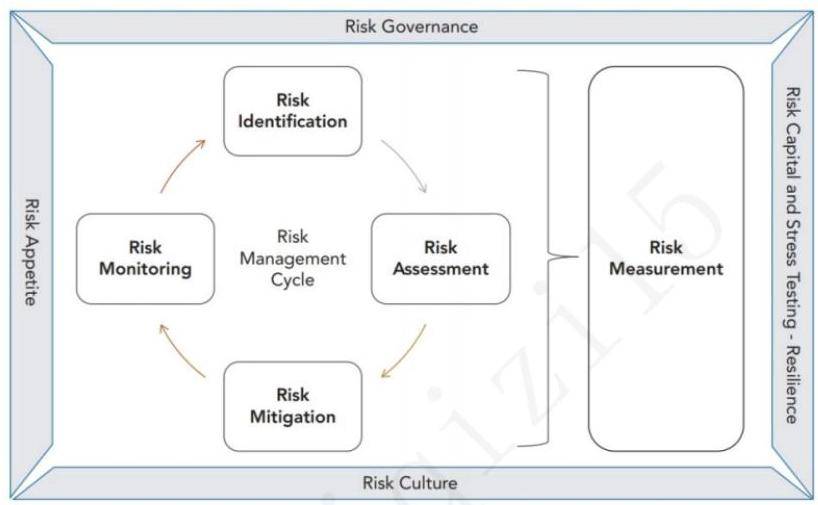
\includegraphics[width=0.5\textwidth]{images/ERMframework.jpg}
        \caption{ERMframework}
        \label{fig:label8}
        \end{figure}
    
    \end{itemize}
\end{itemize}


\subsubsection{Risk governance}
\begin{itemize}
\item Risk governance prescribes the roles and responsibilities of individuals in the three lines of defense, and organizes decision-making and reporting, generally through committees.


    \begin{figure}[H]
    \centering
    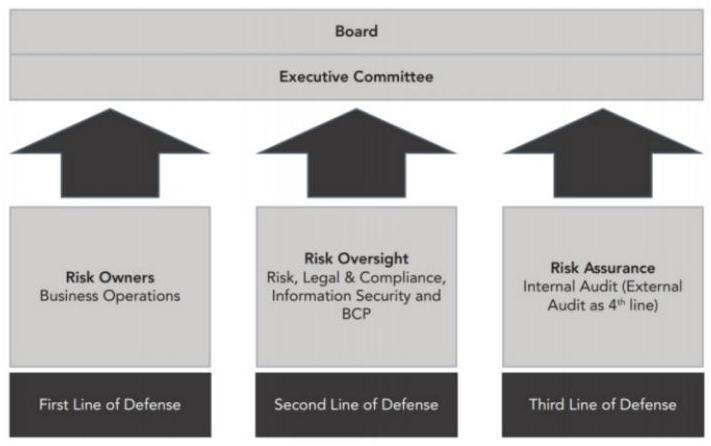
\includegraphics[width=0.5\textwidth]{images/Riskgovernance.jpg}
    \caption{Riskgovernance}
    \label{fig:label9}
    \end{figure}
\end{itemize}



\subsubsection{Risk culture }
\begin{itemize}
\item Corporate culture has a direct influence on the attitude and preferences of the firm when managing risks, from prudent to daring, from compliant to challenging.
\item Regulators consider risk culture to be a key driver of ERM framework effectiveness.
\end{itemize}


\subsubsection{Risk appetite}
\begin{itemize}
\item At the ERM level, risk appetite is typically expressed in overarching risk appetite statements (or policy).
\end{itemize}


\subsubsection{Role of regulatory capital}
\begin{itemize}
\item The objective of the BCBS prudential regulation is threefold:
    \begin{enumerate}
    \item To ensure the solvency and soundness of all financial intermediaries
    \item To provide customers protection from undue risks (failure, fraud, opportunistic behavior)
    \item To promote the efficient and competitive performance of financial institutions
    \end{enumerate}
\item Objective 1 is the primary objective, which is addressed through regulatory capital requirements.
\item Objective 2 and 3 are attained through requirements on the bank's senior management's history and competence (the "fit and proper" criteria), monitoring and reporting on the bank's activities.
\item However, in the United States, the focus has now shifted from capital estimation to stress testing.
    \begin{itemize}
    \item Models developed for the Federal Reserve's Comprehensive Capital Analysis and Review (CCAR) program.
    \item Stress testing requires institutions to estimate expected losses under specific adverse economic.
    \item Capital is a through-the-cycle concept, whereas stress testing is a point-in-time exercise.
    \end{itemize}

\end{itemize}


\subsubsection{Role of economic capital }
\begin{itemize}
\item Financial intermediaries need to calculate economic capital for themselves that fully reflect their risk profile and potential needs to cover unexpected losses.
\item The level of economic capital is largely linked to the credit rating, which then influences their cost of funds.
    \begin{itemize}
    \item The larger the capital, the bigger the buffer against losses, the better the creditworthiness of the institution, the lower the costs of raising funds.
    \end{itemize}
    
\end{itemize}


\subsubsection{Risk aggregation for capital assessment}
\begin{itemize}
\item The aggregation of the different risk classes is the inter-risk diversification.
    \begin{itemize}
    \item  It supplements the intra-risk diversification, which is the diversification within each risk class.
    \end{itemize}
\item Total aggregated capital tends to be lower than the sum of each stand-alone capital amount for individual risk. The difference reflects the diversification benefits.
\item Operational risk can bring important diversification benefits to the total capital.
    \begin{itemize}
    \item Because operational risk typically has a low correlation to other types of financial risks, due to its different risk drivers.
    \end{itemize}
\end{itemize}



\subsubsection{Stress testing}
\begin{itemize}
\item It involves stressing that system or entity beyond normal operation, often to a "breaking point," to observe the results.
    \begin{itemize}
    \item The ultimate objective is to ensure that institutions can absorb the losses incurred under extreme adverse scenarios and remain a going concern.
    \item Stress testing alerts the management to adverse unexpected outcomes and provides an indication of how much capital might be needed to absorb losses.
    \end{itemize}
\end{itemize}


\subsubsection{Stress-testing taxonomy-two dimensions}
\begin{itemize}
\item Dimension 1: Quantitative-Qualitative Approach
    \begin{itemize}
    \item On the quantitative end of the spectrum, stress-testing approaches relate to the sensitivity of models to parameter shocks.
    \item On the qualitative end of the spectrum lie approaches more focused on scenario analysis such as macro stress testing, and non-model-based evaluations like reverse stress testing.
    
    \end{itemize}
\item Dimension 2: Measurable-Immeasurable Risk
    \begin{itemize}
    \item Range from fact-based probabilistic analysis of measurable risks to more hypothetical possibilistic analysis of immeasurable risk.
        \begin{itemize}
        \item On the immeasurable risk end of the spectrum, review and analyze possible risks that are "unknown unknowns". The probability cannot be known, and it cannot be determined which event is more likely than the other.
        
        \end{itemize}
        
    \end{itemize}
    
\end{itemize}


\subsubsection{Parameter stress testing }
\begin{itemize}
\item Parameter (or model) stress testing relates to testing the robustness of a model by changing the value of its parameters.
    \begin{itemize}
    \item It utilizes quantitative approaches and seeks to analyze measurable risks.
    \item Banks will stress model parameters or conduct sensitivity testing to determine the impact on a particular model, portfolio, or the bank.
    \end{itemize}
    
\end{itemize}


\subsubsection{Macroeconomic stress testing}
\begin{itemize}
\item It takes the most holistic view of risk run bank-wide for all risk types: seek to stress both measurable and immeasurable risks, and ideally to stress the dependency structure.
    \begin{itemize}
    \item Macroeconomic scenarios relate to inflation,
    unemployment rate, GDP changes and so forth, and aim at testing the financial resilience of the largest banks.
    \item G-SIBs (globally systemically important banks) are provided a list of macro shock scenarios to assess the solvency level.
    \end{itemize}
\end{itemize}


\subsubsection{Parameter and macroeconomic stress testing}
\begin{itemize}
\item Quantitative analysis:
    \begin{itemize}
    \item Quantitative analysis of parameter stress testing focus on statistical scenarios such as a "standard deviation event" .
    \item Quantitative analysis of macroeconomic stress testing focuses on estimating the output of the models based on a set of macroeconomic scenarios.
    
    \end{itemize}
\end{itemize}


\subsubsection{Reverse stress testing}
\begin{itemize}
\item Reverse stress testing utilizes primarily qualitative approaches and seeks to analyze immeasurable risks.
    \begin{itemize}
    \item It starts from the identification of a pre-defined outcome and then determines how bad an adverse scenario would need to be to achieve the pre-defined outcome.
    \end{itemize}
\item Reverse stress testing is a risk management tool, apt for assessing operational resilience, rather than calculating needed financial resources to weather extreme conditions.
\end{itemize}




\subsubsection{Operational risk stress-testing models}
\begin{itemize}
\item In developing the macroeconomic-based stress-testing models, banks can model either total operational risk losses, or the two components of operational risk losses: frequency and severity (a preferred approach).
    \begin{itemize}
    \item Severity can be more complex to model than frequency as severity is highly impacted by tail events.
    \end{itemize}
\item Once the model produces stressed losses, an expert refinement needs to be performed using scenario analysis.
\end{itemize}





